
\textit{Определение} \textbf{Денежный поток} - денежные поступления и выплаты, которые происходят в течение определенного периода времени в результате бизнес-операций компании или инвестиционной деятельности. 
Он представляет собой выручку, которая остается после вычета всех расходов из общего объема поступлений. 

Денежный поток может быть положительным, если поступления превышают расходы, или отрицательным, если расходы превышают поступления. 
Для бизнеса денежный поток является ключевым показателем его финансового состояния и управления ликвидностью. Для инвесторов он служит основой для оценки доходности инвестиций и оценки риска. 

Денежный поток можно разделить на три основные категории:
\begin{itemize}
    \item Операционный денежный поток связанны с основной деятельностью компании
    \item Инвестиционный денежный поток связанны с инвестиционными операциями
    \item Финансовый денежный поток связанны с финансовыми операциями
\end{itemize}

Примеры классификации денежного потока
\begin{center}
    \begin{tabular}{ |c|c|} 
    Тип поток & Пример \\
     \hline
     Операционный  &  продажи товаров или услуг, оплата заработной платы, закупка инвентаря  \\ 
     Инвестиционный &приобретение или продажа активов, капитальные вложения \\ 
     Финансовый & такими как погашение или выпуск кредитов и облигаций, выплата дивидендов \\ 
     \hline
    \end{tabular}
\end{center}


\textit{Определение} \textbf{Денежная масса} - совокупный объем наличных денег и денежных средств, находящихся в обращении в экономике страны в определенный момент времени. 
Она включает в себя различные формы денег, такие как монеты, банкноты, депозиты наличности в банках и другие ликвидные активы, которые могут быть легко использованы для совершения платежей или обмена на товары и услуги.

Денежная масса измерена различными способами:
\begin{itemize}
    \item  Наличные деньги $M_0$: банкноты и монеты в обращении, находящиеся вне банковской системы.
    \item Широкая денежная масса $M_2$: включает $M0$ и депозиты наличности в коммерческих банках, чековые счета и другие формы ликвидных активов.
\end{itemize}

Контроль и регулирование денежной массы является важным инструментом макроэкономической политики, поскольку она влияет на уровень инфляции, процентные ставки, уровень экономической активности и другие аспекты экономики.

\begin{figure}[h]
    \centering
    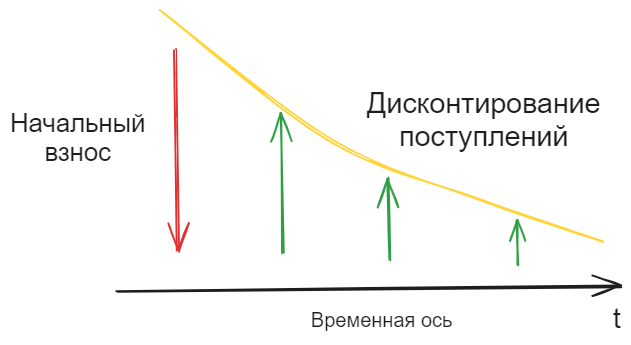
\includegraphics[width=0.5\textwidth]{assets/overview/cash_flow.excalidraw.png}
    \caption{Комбинаторные аукционы подразумевает различие в полезности агента в обладание нескольких товаров}
    \label{npv}
\end{figure}


\textit{Определение} \textbf{Чистая произведения стоимость} - сумма дисконтированных значений потока платежей.

$$
    NPV = \sum_{t=0}^N \frac{CF_T}{(1+i)^t}
$$
- $CF_t$  - (cash flow) поток денег на момент времени $t$ \ref{npv}.  
Принято также выделять начальную инвестицую $IC$ (invested capital):

$$
    NPV = -IC + \sum_{t=1}^N 
$$

Cтавка рефинансирования задает ставку кредитования в банках. 
